\documentclass[aps,prb,twocolumn,amsfonts,showpacs,letterpaper]{revtex4}
\pdfoutput=1
\usepackage{amsmath}  % <- You need this package for 'align' environment
\usepackage{graphicx}  %<-  You need this package to insert graphics
\usepackage[nottoc]{tocbibind}
\usepackage{float}

\begin{document}
	\title{Parameter Optimization of Electric Potential Over Relaxation Solving Method}
	\author{John Rackham}
	\affiliation{Brigham Young University - Idaho: Physics 385 Student} 
	\date{\today} 

\begin{abstract}
The Jacobi and Gauss-Seidel relaxation methods are commonly used to determine the electric potential for a given system. This work utilizes the Gauss-Seidel method and determines the best parameters for optimization of run time.
\end{abstract}

\maketitle

\section{Introduction}\label{intro}
One of the defining problems of Electricity and Magnetism is the determination of electric potential within non trivial systems. When the system is very symmetrical, or possesses some other characteristic that can be utilized the simplify and reduce the problem enough that an analytical, closed form solution is viable. Most real-life cases, however, do not lend themselves well to closed form solution techniques. The case examined within this work is that of a charged rectangular prism of some arbitrary dimensions  and the scalar electric potential field surrounding it.

\section{Methods}
\subsection{Overrelaxation}
When a closed form solution is not readily available a common method of solving the system is the relaxation method. The electric potential at any given point within the system can be approximated as the average of close points surrounding it.\cite{grif} A computational grid is generated for the space that divides it up in to even increments. The relaxation method then steps through the grid and averages the points around it to determine the potential at that point. This process continues until the system converges. This process can be computationally heavy because the electric potential is only known initially at the boundaries.  The grid is typically defined as zero every where that is not defined by the initial voltage. There are two ways to help alleviate the number of iterations the process must make to converge. The first is to intuitively populate the grid with values ranging from the voltage at the boundaries to zero. This method is not discussed in this work because of the further complexity it adds at the lost of abstraction. The choice of values is very much dependent on the specific system. The second correction is to over relax the the system in such a way that speeds up the process. This work uses the over relaxation.

\subsection{Jacobi and Gauss-Seidel Algorithms}
The algorithm to modify the grid is concise. The Jacobi algorithm calculates the average using only the old values and generates a new list in the process. This is suboptimal because the grid must be copied every full iteration. The copying process uses a lot of computational resources particularly as the grid size increases. The Gauss-Seidel algorithm instead steps through the grid and uses the updated values in the subsequent calculations. Because of this the Gauss-Seidel is more efficient and faster than the Jacobi method by a factor of two \cite{gio}.
\begin{multline}
V_{new}(i,j) = \frac{1}{4}[V_{old}(i+1,j) + V_{new}(i-1,j)\\ + V_{old}(i,j+1) + V_{new}(i,j-1)]
\end{multline}

With the overrelaxtion correction applied the algorithm now becomes

\begin{multline}
V_{new}(i,j) = \frac{1+\omega}{4}[V_{old}(i+1,j) + V_{new}(i-1,j)\\ + V_{old}(i,j+1) + V_{new}(i,j-1)-\omega*V_{old}(i,j)]
\end{multline}

where $\omega$ is the parameter that determines how much the alorighm anticipates the value and reduces the number of full iterations across the grid when compared to the normal relaxation method.

\section{Case of a Charged Rectangular Prism}
The case studied in this work comprises of a simple rectangular prism with an electric potential of 100 Volts at the surface. The Gauss-Seidel overrelaxation described above was used and set to stop once the greatest difference between new and old values of $V(i,j)$ was less than 0.001 Volts. Figure 1 shows a cross sectional area of the system of a plane parallel to the x, y, or z axis and containing the rectangular prism.

\begin{figure}[H]
\centering
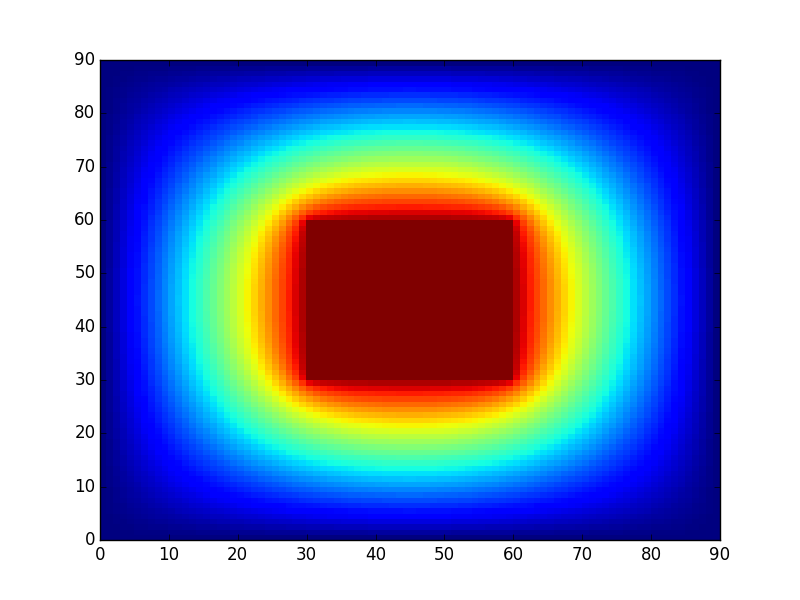
\includegraphics[scale=0.35]{voltage.png}
\caption{cross section of the electric potential field}
\label{Voltage}
\end{figure}

the overrelaxed Gauss-Seidel method yields a result that conform to expected values.

\section{Optimization}
The efficiency of algorithms is conventionall described with big O notation. The methods used in this work is $O(n^{2m})$ where n is determined by the dimensions of the grid and m is the number of iterations needed to converge. The figure of merit for optimizing the algorithm used is the $\omega$ parameter. The only way found to increase the efficiency of the algorithm is to lower the m value. This still leaves the process in the regime of $O(n^{2m})$ but does reduce the over all running time. The case was analysized multiple times using a sequence of $\omega$ values and compared to the number of iterations needed to meet the convergence requirement of the algorithm

\begin{figure}[H]
\centering
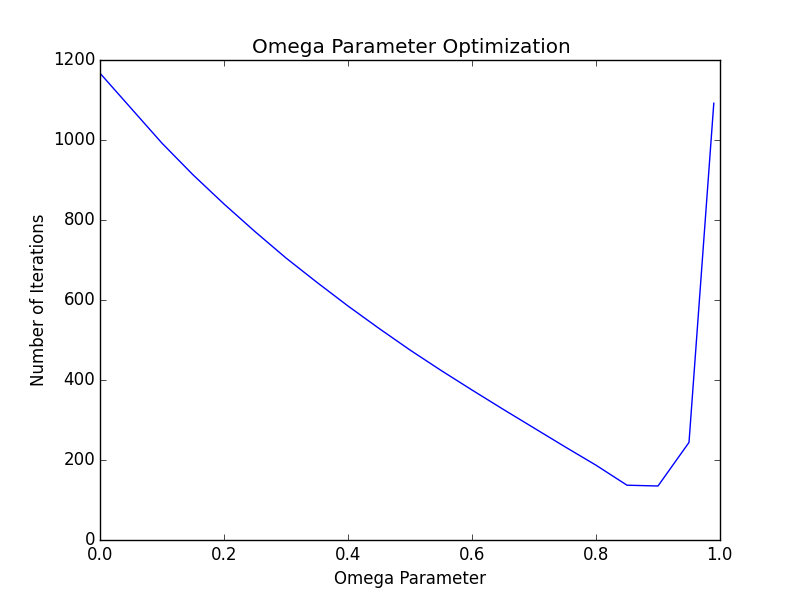
\includegraphics[scale=0.35]{omega.png}
\caption{Omega Values versus Number of Iterations}
\end{figure}

the definition the omega value should be between 0 and 1. The over all trend indicates that that the optimal value of $\omega$ lies  between 0.8 and 0.95. This is similar to other findings in the field.\cite{new}. A focused of figure of the rregion finds the optimal value to be near 0.87.

\begin{figure}[H]
\centering
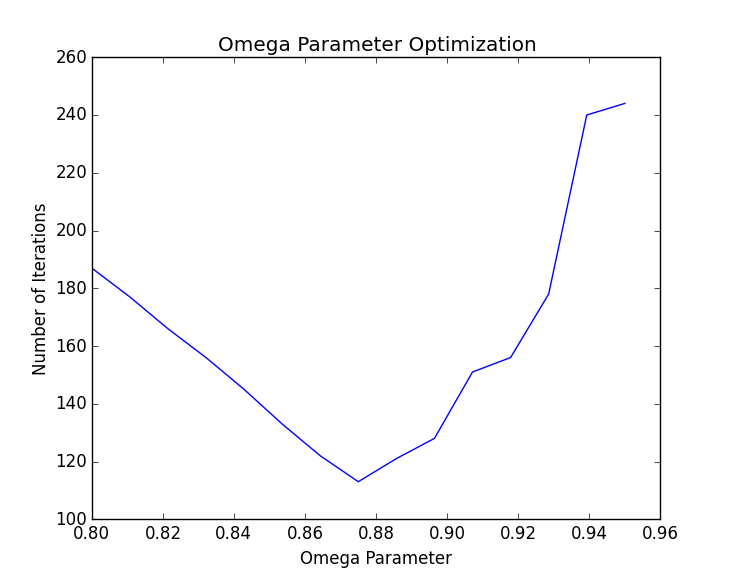
\includegraphics[scale=0.35]{omega2.png}
\caption{Omega Values versus Number of Iterations}
\end{figure}

\section{Conclusion}

The Overrelaxed Gauss-Seidel method is more efficient than the Jacobi and yields results inline with expected values. By optimizing the $\omega$ parameter one can significantly reduce the number of total iterations and shorten the run time of the process.

\bibliography{refs}

\end{document}





